%%____________________________________________________________________________||
\section{Interpretations with simplified ``split SUSY'' models}
\label{app:LLP}

\subsection{Distributions}
\label{app:LLP-distributions}

Figure \ref{fig:T1qqqqLLvsT1qqqqLL} shows a comparison of the distributions of 
the main kinematic variables between various \ctau models. In general, the
distributions become softer with increasing lifetime. % as the jet response and
%reconstruction efficiency fall with increasing displacement from the primary
%vertex. In addition, the gluinos become more likely to decay outside the detector.
There is also an enhancement in the number of b-tagged jets when \ctau
is of order 1~mm. This enhancement is less noticeable for compressed models
as the displaced jets are softer and therefore more likely to be below the jet 
\pt threshold.

Figure \ref{fig:T1qqqqLLvsT1qqqq} shows a comparison of the kinematic
distributions between the prompt (FastSim) T1qqqq model and the
T1qqqqLL model with a relatively prompt lifetime of \ctau$=0.001$~mm. 
The two samples show reasonable agreement.

Figure \ref{fig:T1qqqqLLvsT1bbbb} shows a comparison of the kinematic
distributions between the \ctau$=1$~mm model and the T1bbbb model. The two
models have similar kinematics. There is some difference in the \nb distribution
that arises from the difference in b-tagging efficiency for b jets and
displaced jets. This difference becomes larger with decreasing jet \pt, as
seen in Sec.~\ref{app:LLP-btagging}, and is thus more noticeable
for the compressed samples.

\begin{figure}[h!]
  \begin{center}
    \subfigure{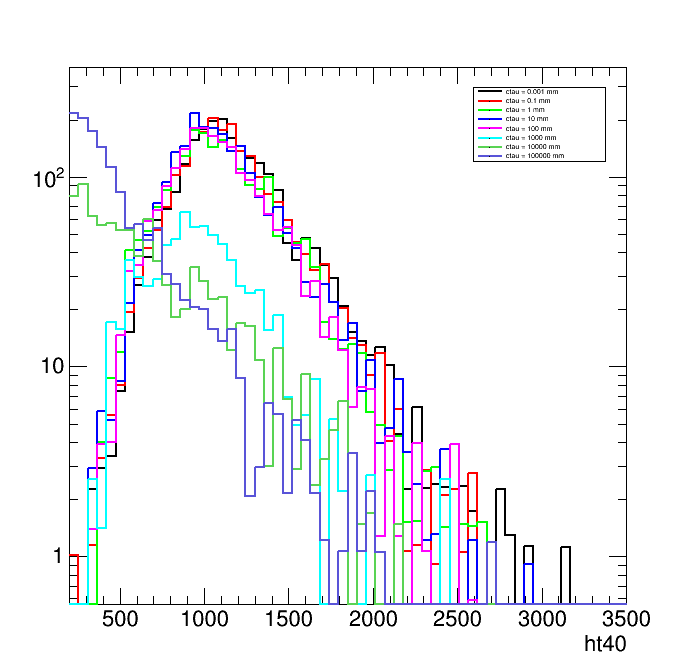
\includegraphics[width=0.28\textwidth]{figures/LLPResults/T1qqqqLL_1000_200/ht40_all_all}} ~
    \subfigure{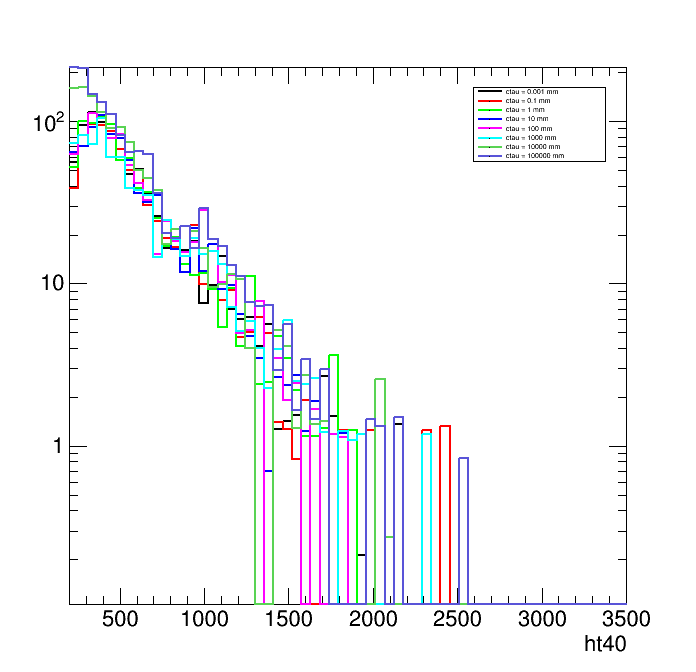
\includegraphics[width=0.28\textwidth]{figures/LLPResults/T1qqqqLL_1000_900/ht40_all_all}} \\
    \subfigure{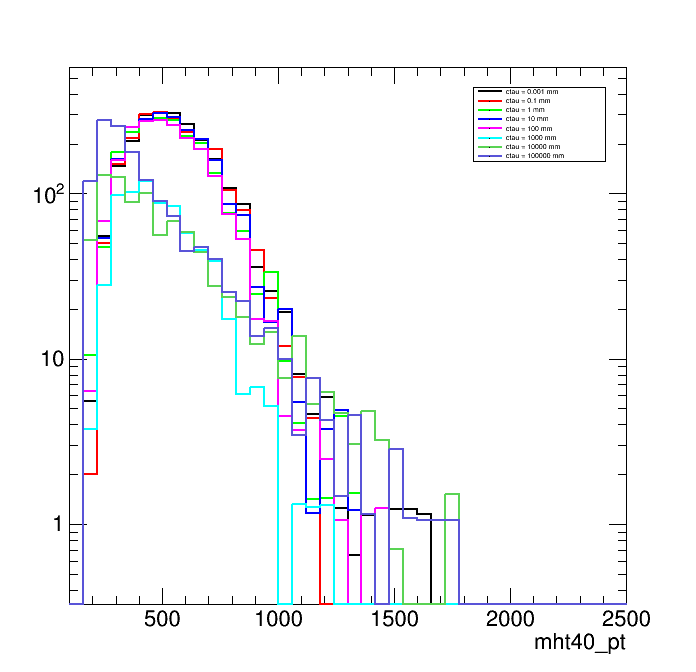
\includegraphics[width=0.28\textwidth]{figures/LLPResults/T1qqqqLL_1000_200/mht40_pt_all_all}} ~
    \subfigure{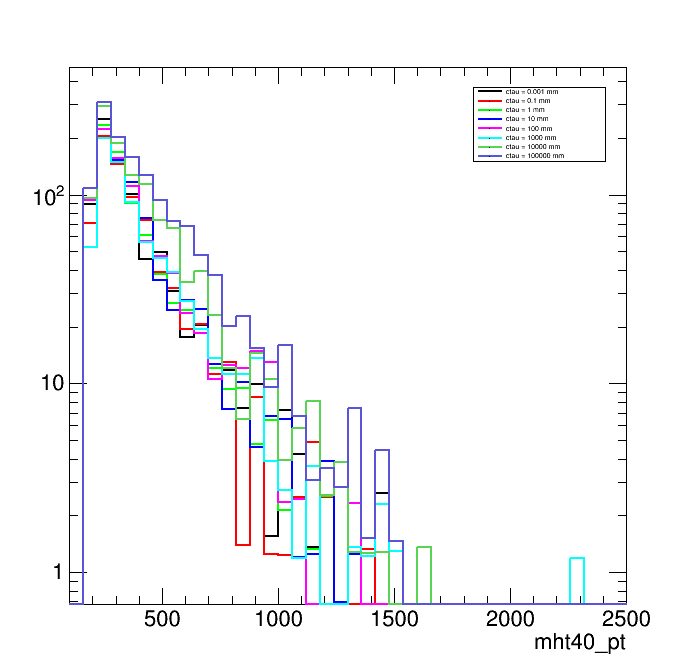
\includegraphics[width=0.28\textwidth]{figures/LLPResults/T1qqqqLL_1000_900/mht40_pt_all_all}} \\
    \subfigure{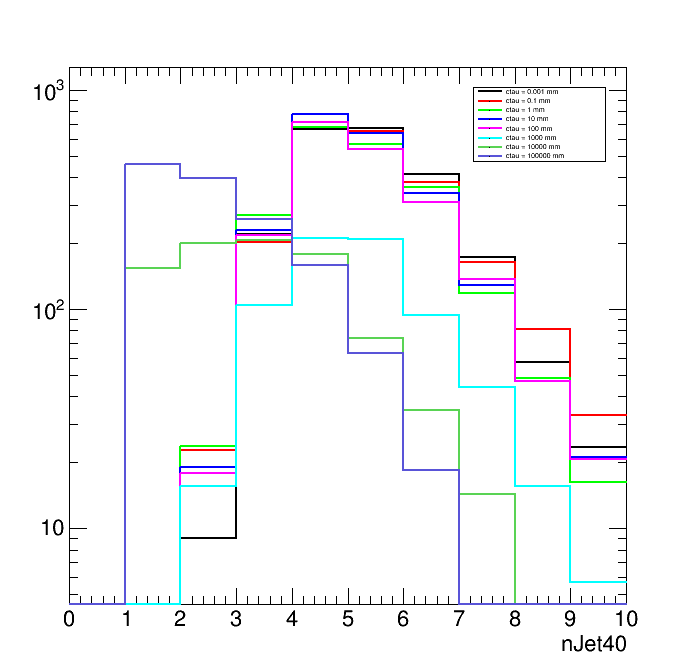
\includegraphics[width=0.28\textwidth]{figures/LLPResults/T1qqqqLL_1000_200/nJet40_all_all}} ~
    \subfigure{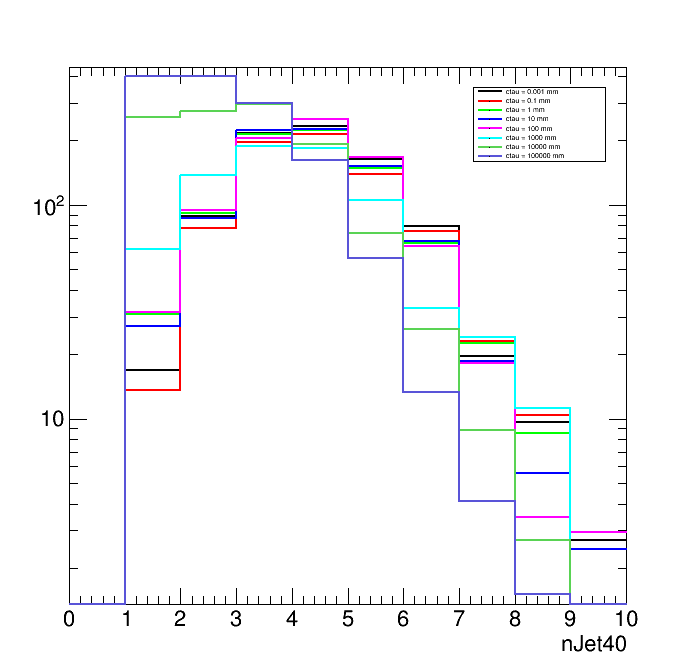
\includegraphics[width=0.28\textwidth]{figures/LLPResults/T1qqqqLL_1000_900/nJet40_all_all}} \\
    \subfigure{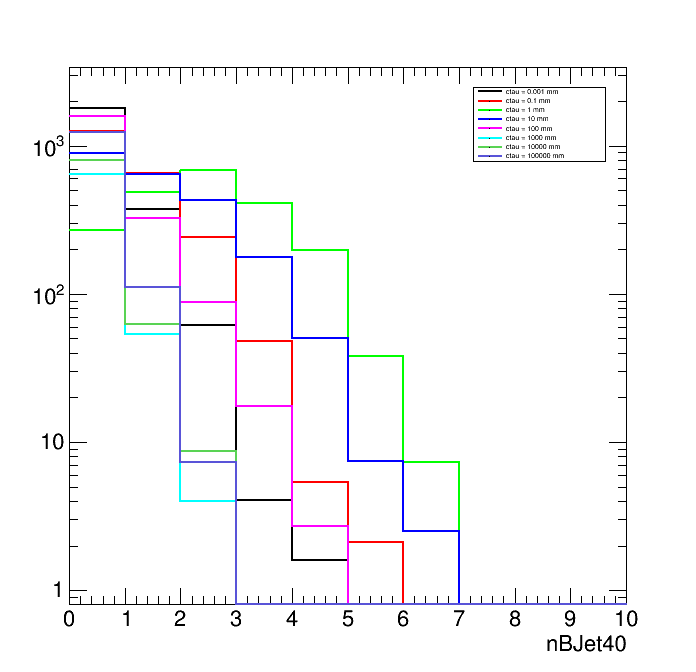
\includegraphics[width=0.28\textwidth]{figures/LLPResults/T1qqqqLL_1000_200/nBJet40_all_all}} ~
    \subfigure{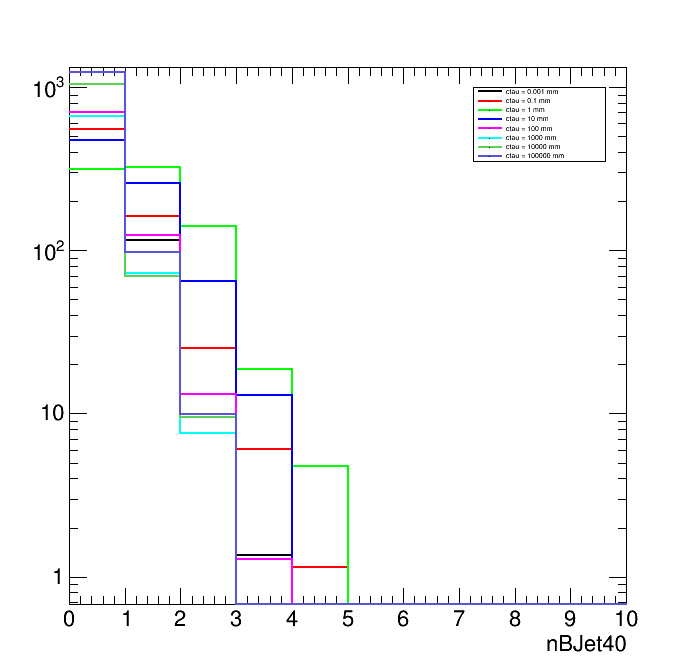
\includegraphics[width=0.28\textwidth]{figures/LLPResults/T1qqqqLL_1000_900/nBJet40_all_all}}
    \caption{Kinematic distributions comparing various lifetimes, for an uncompressed (1000,200) (Left)
        and compressed (1000,900) (Right) mass point.}
    \label{fig:T1qqqqLLvsT1qqqqLL}
  \end{center}
\end{figure}

\begin{figure}[h!]
  \begin{center}
    \subfigure{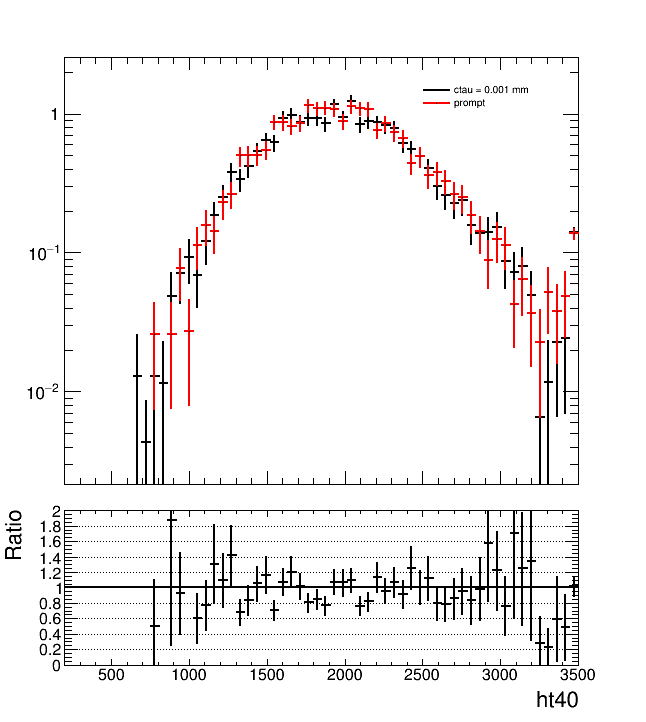
\includegraphics[width=0.28\textwidth]{figures/LLPResults/T1qqqqLL_vs_T1qqqq_1800_200/ht40_all_all}} ~
    \subfigure{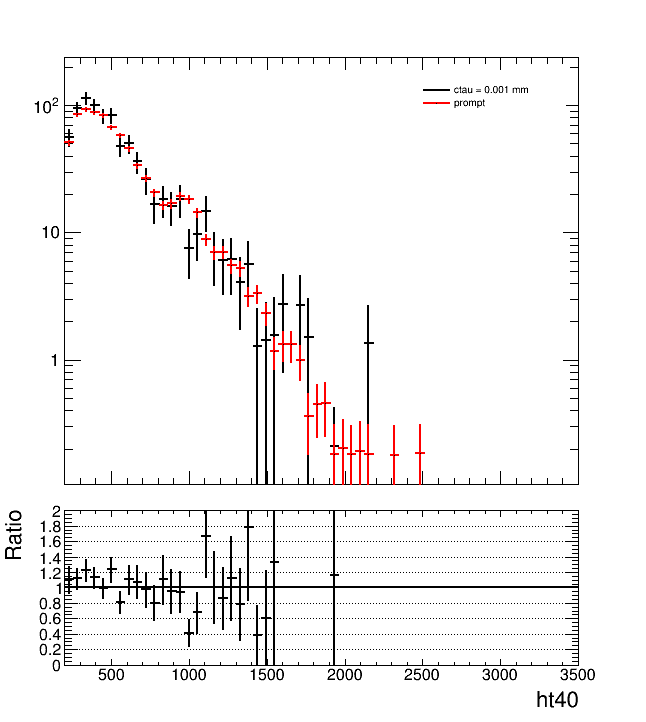
\includegraphics[width=0.28\textwidth]{figures/LLPResults/T1qqqqLL_vs_T1qqqq_1000_900/ht40_all_all}} \\
    \subfigure{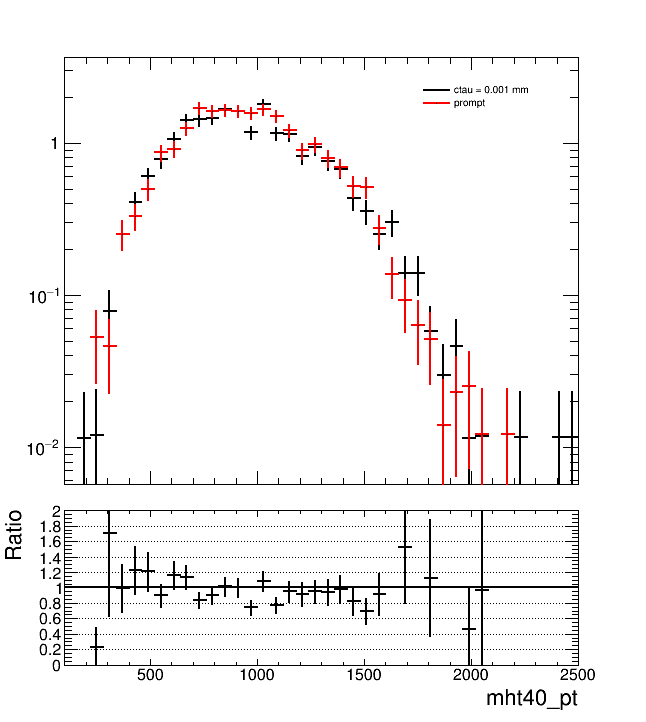
\includegraphics[width=0.28\textwidth]{figures/LLPResults/T1qqqqLL_vs_T1qqqq_1800_200/mht40_pt_all_all}} ~
    \subfigure{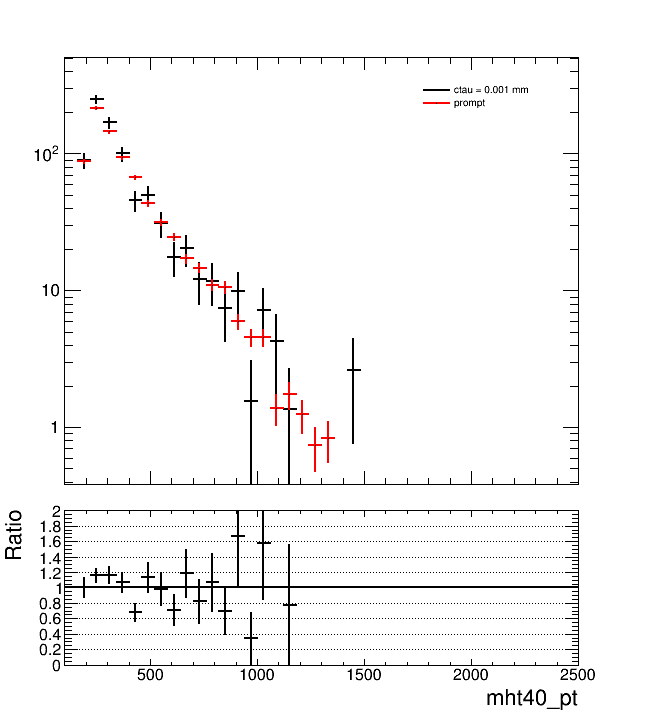
\includegraphics[width=0.28\textwidth]{figures/LLPResults/T1qqqqLL_vs_T1qqqq_1000_900/mht40_pt_all_all}} \\
    \subfigure{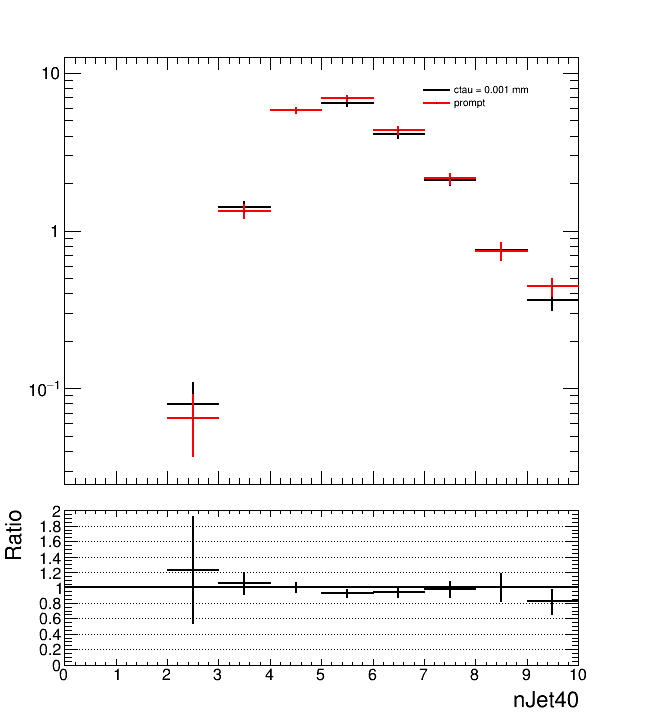
\includegraphics[width=0.28\textwidth]{figures/LLPResults/T1qqqqLL_vs_T1qqqq_1800_200/nJet40_all_all}} ~
    \subfigure{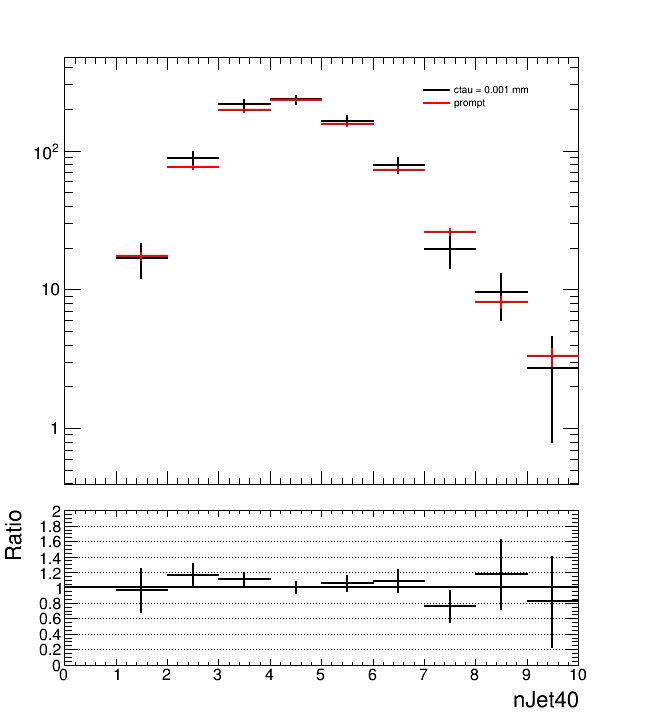
\includegraphics[width=0.28\textwidth]{figures/LLPResults/T1qqqqLL_vs_T1qqqq_1000_900/nJet40_all_all}} \\
    \subfigure{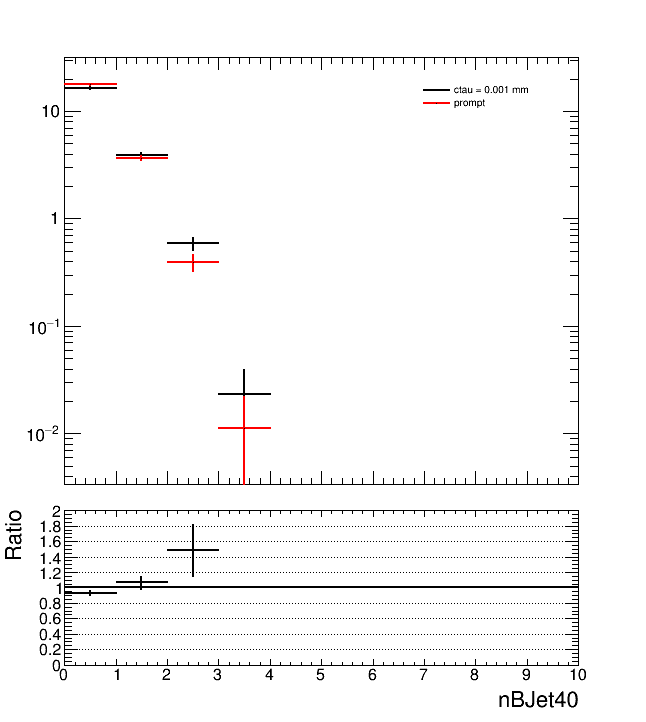
\includegraphics[width=0.28\textwidth]{figures/LLPResults/T1qqqqLL_vs_T1qqqq_1800_200/nBJet40_all_all}} ~
    \subfigure{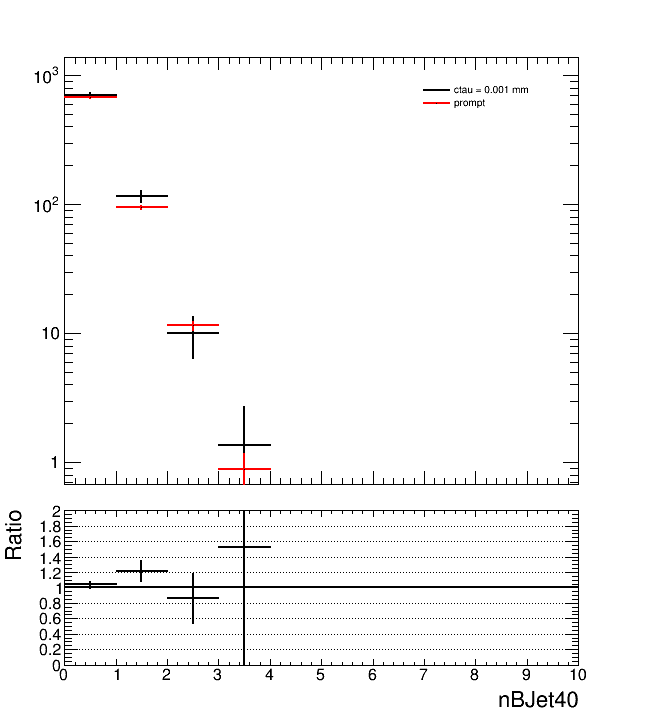
\includegraphics[width=0.28\textwidth]{figures/LLPResults/T1qqqqLL_vs_T1qqqq_1000_900/nBJet40_all_all}}
    \caption{Kinematic distributions comparing prompt T1qqqq and T1qqqqLL with \ctau$=0.001$~mm, for an 
        uncompressed (1800,200) (Left) and compressed (1000,900) (Right) mass point.}
    \label{fig:T1qqqqLLvsT1qqqq}
  \end{center}
\end{figure}

\begin{figure}[h!]
  \begin{center}
    \subfigure{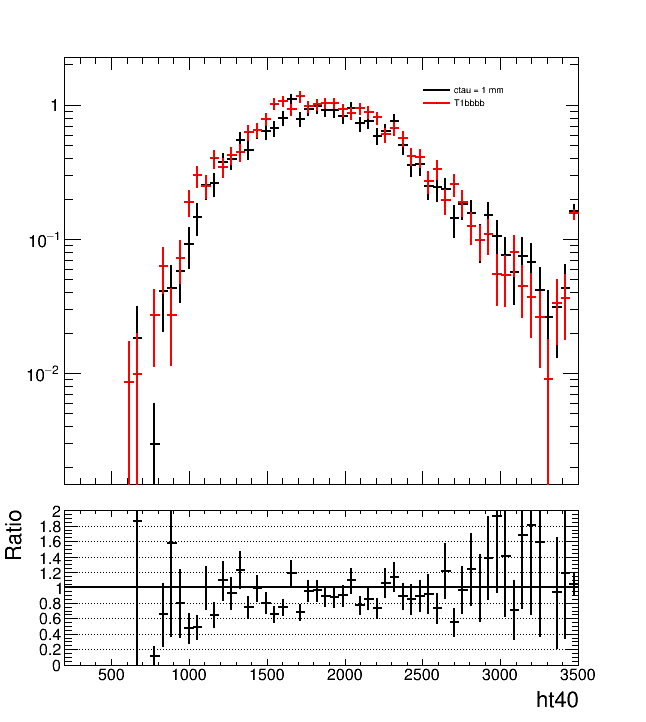
\includegraphics[width=0.28\textwidth]{figures/LLPResults/T1qqqqLL_vs_T1bbbb_1800_200/ht40_all_all}} ~
    \subfigure{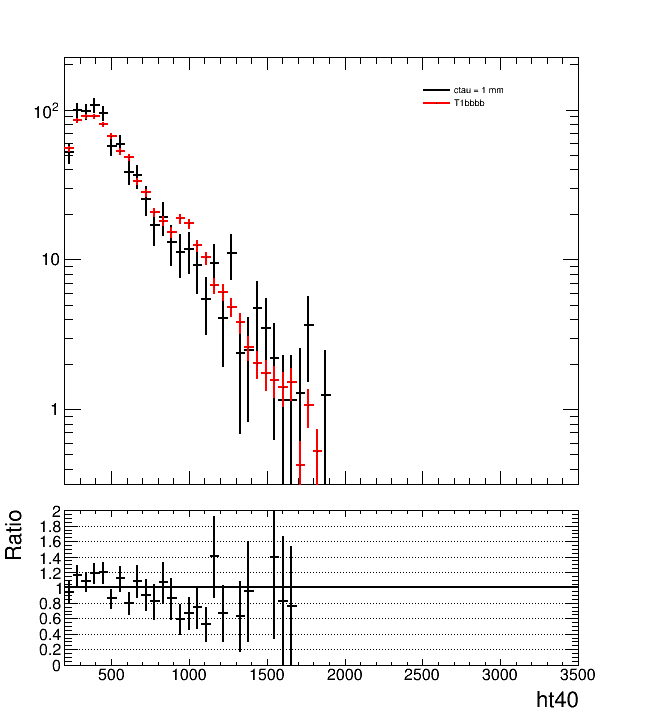
\includegraphics[width=0.28\textwidth]{figures/LLPResults/T1qqqqLL_vs_T1bbbb_1000_900/ht40_all_all}} \\
    \subfigure{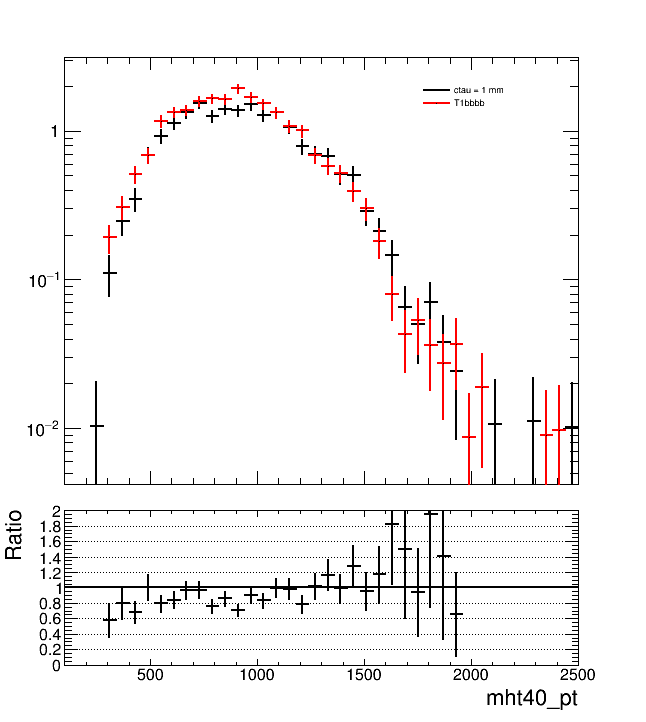
\includegraphics[width=0.28\textwidth]{figures/LLPResults/T1qqqqLL_vs_T1bbbb_1800_200/mht40_pt_all_all}} ~
    \subfigure{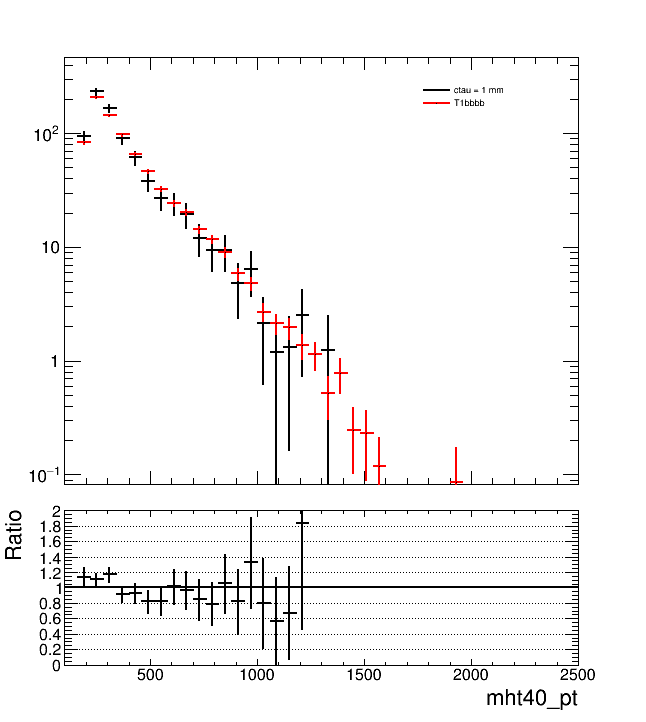
\includegraphics[width=0.28\textwidth]{figures/LLPResults/T1qqqqLL_vs_T1bbbb_1000_900/mht40_pt_all_all}} \\
    \subfigure{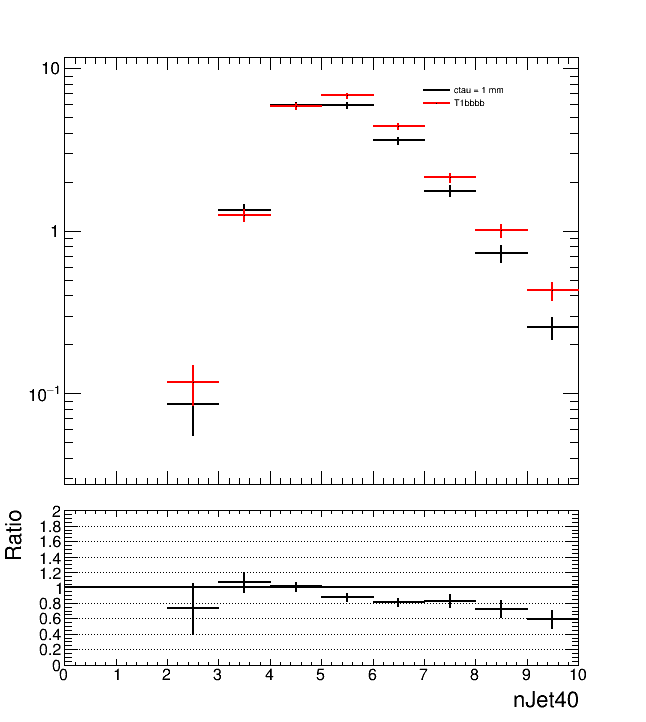
\includegraphics[width=0.28\textwidth]{figures/LLPResults/T1qqqqLL_vs_T1bbbb_1800_200/nJet40_all_all}} ~
    \subfigure{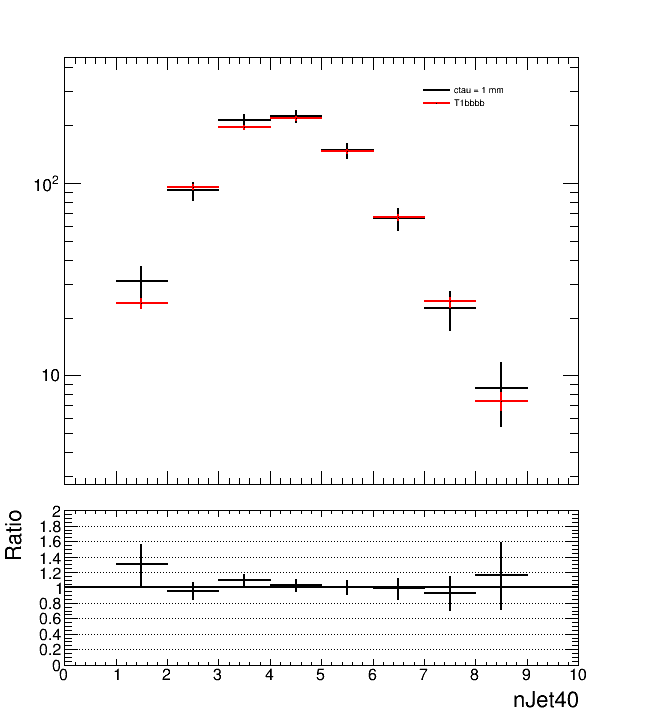
\includegraphics[width=0.28\textwidth]{figures/LLPResults/T1qqqqLL_vs_T1bbbb_1000_900/nJet40_all_all}} \\
    \subfigure{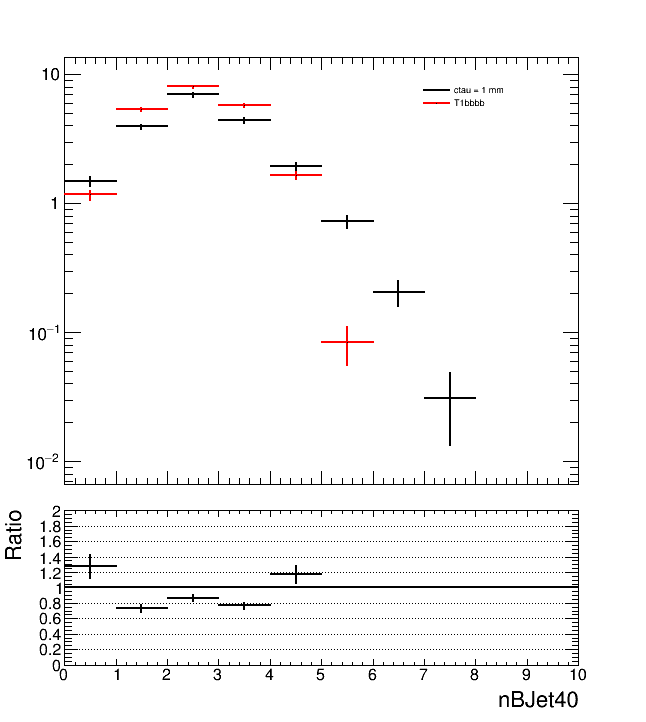
\includegraphics[width=0.28\textwidth]{figures/LLPResults/T1qqqqLL_vs_T1bbbb_1800_200/nBJet40_all_all}} ~
    \subfigure{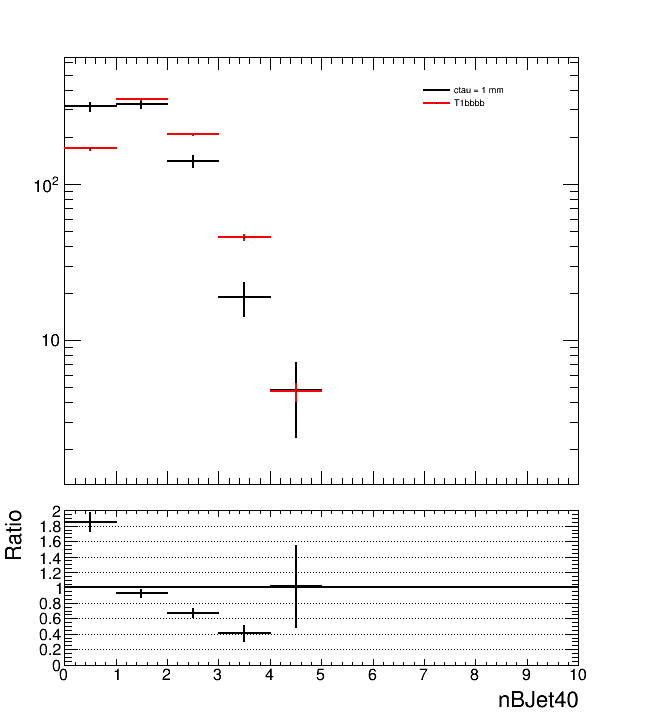
\includegraphics[width=0.28\textwidth]{figures/LLPResults/T1qqqqLL_vs_T1bbbb_1000_900/nBJet40_all_all}}
    \caption{Kinematic distributions comparing prompt T1bbbb and T1qqqqLL with \ctau$=1$~mm, for an
        uncompressed (1800,200) (Left) and compressed (1000,900) (Right) mass point.}
    \label{fig:T1qqqqLLvsT1bbbb}
  \end{center}
\end{figure}

\subsection{Trigger and jet ID}
\label{app:LLP-trigger}
%
%Table \ref{tab:LLP-triggereff} shows the efficiency of the signal region 
%triggers (listed in Sec.~\ref{sec:triggers}) for some representative mass points
%and various lifetimes. Some comment about magnitude of inefficiency, related to
%jet id requirement in trigger.
%
%Table goes here.
%
%A trigger requirement is imposed on these signal models according to the
%trigger emulation provided in the simulation samples. A systematic uncertainty
%is assigned that is dependent on \mht and \njet. These uncertainties are taken 
%from the efficiencies measured in data, as described in Sec.~\ref{sec:triggers}.

The efficiency of the trigger and the event veto for jets failing ID are found
to be reasonably high. These are summarised for three benchmark models in 
Tables~\ref{tab:cut_flow_ctau_0p001}-\ref{tab:cut_flow_ctau_100000}. More detailed material will be provided soon.

\subsection{Jet response}
\label{app:LLP-jetresponse}

Figure \ref{fig:T1qqqq:response} shows the jet response (defined as the ratio
of reconstructed \pt to generator-level \pt) for generator jets with $\pt>40$ and 
$|\eta|<2.4$ for the different lifetimes considered.

\begin{figure}
    \begin{center}
    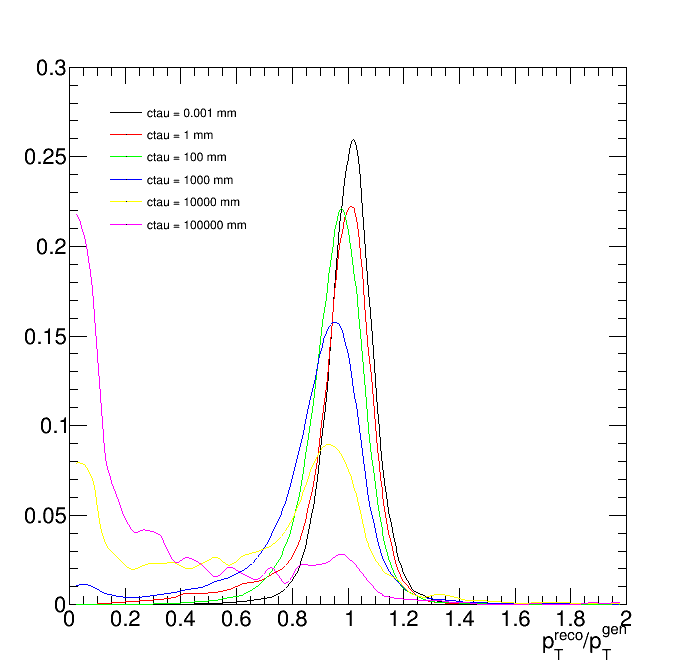
\includegraphics[width=0.6\textwidth]{figures/LLPResults/T1qqqqLL_response}
    \caption{Distribution of response for generator-level jets with $\pt>40$ and $|\eta|<2.4$,
        for various \ctau models. Only jets originating from one of the long-lived gluinos
        and that are matched to a reconstructed jet are considered.}
    \label{fig:T1qqqq:response}
    \end{center}
\end{figure}

\subsection{b-tagging}
\label{app:LLP-btagging}

Documentation in progress. See slides and email exchange with BTV on the
hypernews for the agreement that was reached in terms of b-tag scale factors 
and associated uncertainties.

